\subsubsection{Heurísitca de Savings}

\subsubsubsection{Medición en base al tamaño del grafo}

Al comienzo de su ejecución, la herurística calcula el saving entre todo par de nodos, para luego recorrer cada uno de ellos para construir la solución final. Es de esperar entonces que savings presente una curva cuya pendiente incremente a medida que crece el valor de n.

\begin{figure}[H]
	\centering
	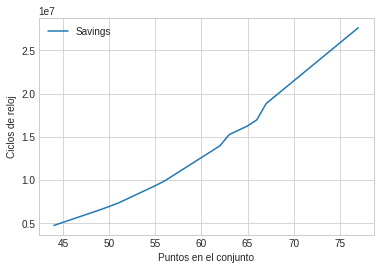
\includegraphics[scale=0.6]{exercise5/savings3.png}
\end{figure}

El gráfico cumple con lo esperado y presenta una curva consistente con la creciente cantidad de puntos y la complejidad $\mathcal{O}(n^{3})$ de la heurística.